\begin{scriptsize}
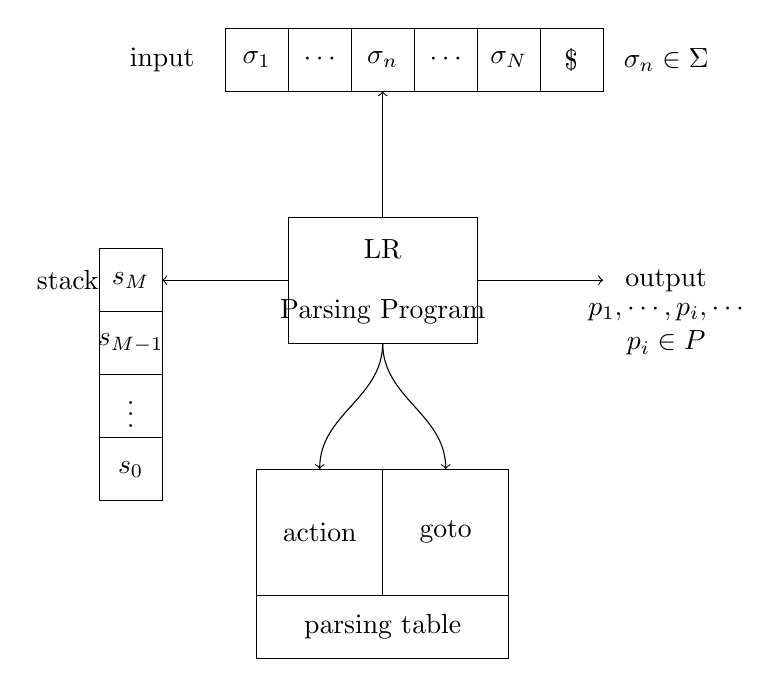
\begin{tikzpicture}
  [x=4mm,y=4mm,node distance=1,
    dati/.style={rounded corners,draw},
    box/.style={draw},
    stgrid/.style={draw=#1,},
    agrid/.style={stgrid=black!10},
    bgrid/.style={stgrid=cyan!50},
]

  \draw[box] (-3,-2)--(-3,2)--(3,2)--(3,-2)--cycle;
  \node(lr) at (0,1) {LR};
  \node(pp) at (0,-1) {Parsing Program};

  \draw[box] (-5,6)--(-3,6)--(-3,8)--(-5,8)--cycle;
  \draw[box] (-3,6)--(-1,6)--(-1,8)--(-3,8)--cycle;
  \draw[box] (-1,6)--( 1,6)--( 1,8)--(-1,8)--cycle;
  \draw[box] ( 1,6)--( 3,6)--( 3,8)--( 1,8)--cycle;
  \draw[box] ( 3,6)--( 5,6)--( 5,8)--( 3,8)--cycle;
  \draw[box] ( 5,6)--( 7,6)--( 7,8)--( 5,8)--cycle;

  \node(input) at (-7,7) {input};
  \node(a1) at (-4,7) {$\sigma_1$};
  \node(a2) at (-2,7) {$\cdots$};
  \node(a3) at ( 0,7) {$\sigma_n$};
  \node(a4) at ( 2,7) {$\cdots$};
  \node(a5) at ( 4,7) {$\sigma_N$};
  \node(a6) at ( 6,7) {\$};
  \node(an) at (9,7) {$\sigma_n\in \Sigma$};

  \node(output) at (9,0) {output};
  \node(output1) at (9,-1) {$p_1,\cdots,p_i,\cdots$};
  \node(output1) at (9,-2) {$p_i\in P$};
  
  \draw[->] (0,2)--(0,6);
  \draw[->] (3,0)--(7,0);
  \draw[->] (-3,0)--(-7,0);

  \draw[box] (-9,-1)--(-7,-1)--(-7,1)--(-9,1)--cycle;
  \draw[box] (-9,-3)--(-7,-3)--(-7,-1)--(-9,-1)--cycle;
  \draw[box] (-9,-5)--(-7,-5)--(-7,-3)--(-9,-3)--cycle;
  \draw[box] (-9,-7)--(-7,-7)--(-7,-5)--(-9,-5)--cycle;
  
  \node(sM) at (-8,0) {$s_M$};
  \node(sM1) at (-8,-2) {$s_{M-1}$};
  \node(sM2) at (-8,-4) {$\vdots$};
  \node(s0) at (-8,-6) {$s_0$};

  \node(stack) at (-10,0) {stack};

  \draw[box] (-4,-6)--(-4,-10)--(0,-10)--(0,-6)--cycle;
  \draw[box] (0,-6)--(0,-10)--(4,-10)--(4,-6)--cycle;
  \draw[box] (-4,-10)--(-4,-12)--(4,-12)--(4,-10)--cycle;
  
  \node(action) at (-2,-8) {action};
  \node(goto) at (2,-8) {goto};
  \node(pt) at (0,-11) {parsing table};

  \draw[->] (0,-2) to[out=270,in=90] (-2,-6);
  \draw[->] (0,-2) to[out=270,in=90] (2,-6);

\end{tikzpicture}
\end{scriptsize}
